% !TeX root = RJwrapper.tex
\title{Rain in Australia. Classification Prediction Model}
\author{by Sumaira Afzal, Viraja Ketkar, Murlidhar Loka, Vadim Spirkov}

\maketitle

\abstract{%
An abstract of less than 150 words.
}

% Any extra LaTeX you need in the preamble

\hypertarget{introduction}{%
\subsection{Introduction}\label{introduction}}

\hypertarget{background}{%
\subsection{Background}\label{background}}

\hypertarget{objective}{%
\subsection{Objective}\label{objective}}

\hypertarget{data-analisys}{%
\section{Data Analisys}\label{data-analisys}}

The data set we are going to use for our research contains daily weather
observations from numerous Australian weather stations from 2007 till
2017. There are over 142000 records. It has been sourced from
\href{https://www.kaggle.com/jsphyg/weather-dataset-rattle-package}{Kagle}

\hypertarget{data-dictionary}{%
\subsection{Data Dictionary}\label{data-dictionary}}

We exclude the variable Risk-MM when training your binary classification
model. If we don't exclude it, you will leak the answers to our model
and reduce its predictability

\begin{longtable}[]{@{}ll@{}}
\toprule
\begin{minipage}[b]{0.52\columnwidth}\raggedright
Column Name\strut
\end{minipage} & \begin{minipage}[b]{0.43\columnwidth}\raggedright
Column Description\strut
\end{minipage}\tabularnewline
\midrule
\endhead
\begin{minipage}[t]{0.52\columnwidth}\raggedright
Date\strut
\end{minipage} & \begin{minipage}[t]{0.43\columnwidth}\raggedright
Date of observation\strut
\end{minipage}\tabularnewline
\begin{minipage}[t]{0.52\columnwidth}\raggedright
Location\strut
\end{minipage} & \begin{minipage}[t]{0.43\columnwidth}\raggedright
Common name of the location of the weather station\strut
\end{minipage}\tabularnewline
\begin{minipage}[t]{0.52\columnwidth}\raggedright
MinTemp\strut
\end{minipage} & \begin{minipage}[t]{0.43\columnwidth}\raggedright
Minimum temperature in degrees Celsius\strut
\end{minipage}\tabularnewline
\begin{minipage}[t]{0.52\columnwidth}\raggedright
MaxTemp\strut
\end{minipage} & \begin{minipage}[t]{0.43\columnwidth}\raggedright
Maximum temperature in degrees Celsius\strut
\end{minipage}\tabularnewline
\begin{minipage}[t]{0.52\columnwidth}\raggedright
Rainfall\strut
\end{minipage} & \begin{minipage}[t]{0.43\columnwidth}\raggedright
Amount of rainfall recorded for the day in mm\strut
\end{minipage}\tabularnewline
\begin{minipage}[t]{0.52\columnwidth}\raggedright
Evaporation\strut
\end{minipage} & \begin{minipage}[t]{0.43\columnwidth}\raggedright
So-called Class A pan evaporation (mm) in the 24 hours to 9am\strut
\end{minipage}\tabularnewline
\begin{minipage}[t]{0.52\columnwidth}\raggedright
Sunshine\strut
\end{minipage} & \begin{minipage}[t]{0.43\columnwidth}\raggedright
Number of hours of bright sunshine in the day\strut
\end{minipage}\tabularnewline
\begin{minipage}[t]{0.52\columnwidth}\raggedright
WindGustDir\strut
\end{minipage} & \begin{minipage}[t]{0.43\columnwidth}\raggedright
Direction of the strongest wind gust in the 24 hours to midnight\strut
\end{minipage}\tabularnewline
\begin{minipage}[t]{0.52\columnwidth}\raggedright
WindGustSpeed\strut
\end{minipage} & \begin{minipage}[t]{0.43\columnwidth}\raggedright
Speed (km/h) of the strongest wind gust in the 24 hours to
midnight\strut
\end{minipage}\tabularnewline
\begin{minipage}[t]{0.52\columnwidth}\raggedright
WindDir9amDirection\strut
\end{minipage} & \begin{minipage}[t]{0.43\columnwidth}\raggedright
Of the wind at 9am\strut
\end{minipage}\tabularnewline
\begin{minipage}[t]{0.52\columnwidth}\raggedright
WindDir3pmDirection\strut
\end{minipage} & \begin{minipage}[t]{0.43\columnwidth}\raggedright
Of the wind at 3pm\strut
\end{minipage}\tabularnewline
\begin{minipage}[t]{0.52\columnwidth}\raggedright
WindSpeed9amWind\strut
\end{minipage} & \begin{minipage}[t]{0.43\columnwidth}\raggedright
Wind speed (km/hr) averaged over 10 minutes prior to 9am\strut
\end{minipage}\tabularnewline
\begin{minipage}[t]{0.52\columnwidth}\raggedright
WindSpeed3pmWind\strut
\end{minipage} & \begin{minipage}[t]{0.43\columnwidth}\raggedright
Wind Speed (km/hr) averaged over 10 minutes prior to 3pm\strut
\end{minipage}\tabularnewline
\begin{minipage}[t]{0.52\columnwidth}\raggedright
Humidity9amHumidity\strut
\end{minipage} & \begin{minipage}[t]{0.43\columnwidth}\raggedright
Humidity (percent) at 9am\strut
\end{minipage}\tabularnewline
\begin{minipage}[t]{0.52\columnwidth}\raggedright
Humidity3pmHumidity\strut
\end{minipage} & \begin{minipage}[t]{0.43\columnwidth}\raggedright
Humidity (percent) at 3pm\strut
\end{minipage}\tabularnewline
\begin{minipage}[t]{0.52\columnwidth}\raggedright
Pressure9amAtmospheric\strut
\end{minipage} & \begin{minipage}[t]{0.43\columnwidth}\raggedright
Pressure (hpa) reduced to mean sea level at 9am\strut
\end{minipage}\tabularnewline
\begin{minipage}[t]{0.52\columnwidth}\raggedright
Pressure3pmAtmospheric\strut
\end{minipage} & \begin{minipage}[t]{0.43\columnwidth}\raggedright
Pressure (hpa) reduced to mean sea level at 3pm\strut
\end{minipage}\tabularnewline
\begin{minipage}[t]{0.52\columnwidth}\raggedright
Cloud9amFraction\strut
\end{minipage} & \begin{minipage}[t]{0.43\columnwidth}\raggedright
Area of sky obscured by cloud at 9am. This is measured in ``oktas'',
which are a unit of eights. It records how many eights of the sky are
obscured by cloud. A 0 measure indicates completely clear sky whilst an
8 indicates that it is completely overcast\strut
\end{minipage}\tabularnewline
\begin{minipage}[t]{0.52\columnwidth}\raggedright
Cloud3pmFraction\strut
\end{minipage} & \begin{minipage}[t]{0.43\columnwidth}\raggedright
Area of sky obscured by cloud (in ``oktas'': eighths) at 3pm. See
Cloud9am for a description of the values\strut
\end{minipage}\tabularnewline
\begin{minipage}[t]{0.52\columnwidth}\raggedright
Temp9amTemperature\strut
\end{minipage} & \begin{minipage}[t]{0.43\columnwidth}\raggedright
Temperature (degrees C) at 9am\strut
\end{minipage}\tabularnewline
\begin{minipage}[t]{0.52\columnwidth}\raggedright
Temp3pmTemperature\strut
\end{minipage} & \begin{minipage}[t]{0.43\columnwidth}\raggedright
Temperature (degrees C) at 3pm\strut
\end{minipage}\tabularnewline
\begin{minipage}[t]{0.52\columnwidth}\raggedright
RainTodayBoolean\strut
\end{minipage} & \begin{minipage}[t]{0.43\columnwidth}\raggedright
Rainy today. 1 if precipitation (mm) in the 24 hours to 9am exceeds 1mm,
otherwise 0\strut
\end{minipage}\tabularnewline
\begin{minipage}[t]{0.52\columnwidth}\raggedright
RISK\_MM\strut
\end{minipage} & \begin{minipage}[t]{0.43\columnwidth}\raggedright
Amount of rain. A kind of measure of the ``risk''. This column is
redundant and will be dropped\strut
\end{minipage}\tabularnewline
\begin{minipage}[t]{0.52\columnwidth}\raggedright
\textbf{RainTomorrowThe}\strut
\end{minipage} & \begin{minipage}[t]{0.43\columnwidth}\raggedright
\textbf{Target variable. Will it rain tomorrow?}\strut
\end{minipage}\tabularnewline
\bottomrule
\end{longtable}

\hypertarget{data-exploration}{%
\subsection{Data Exploration}\label{data-exploration}}

Let's take a close look at the data set. We start with loading weather
observations from the file into a data frame. We remove RISK\_MM as
explained and convert Date column to \emph{date} format

\begin{Schunk}
\begin{Sinput}
weatherData = read.csv("../data/weatherAUS.csv", header = TRUE, na.strings = c("NA","","#NA"),sep=",")
weatherData = subset(weatherData, select = -RISK_MM)
weatherData$Date = as.Date(as.character(weatherData$Date),"%Y-%m-%d")
\end{Sinput}
\end{Schunk}

Now let's load coordinates of the weather stations and have a bird-eye
view of the weather station locations

\begin{Schunk}
\begin{figure}[H]

{\centering 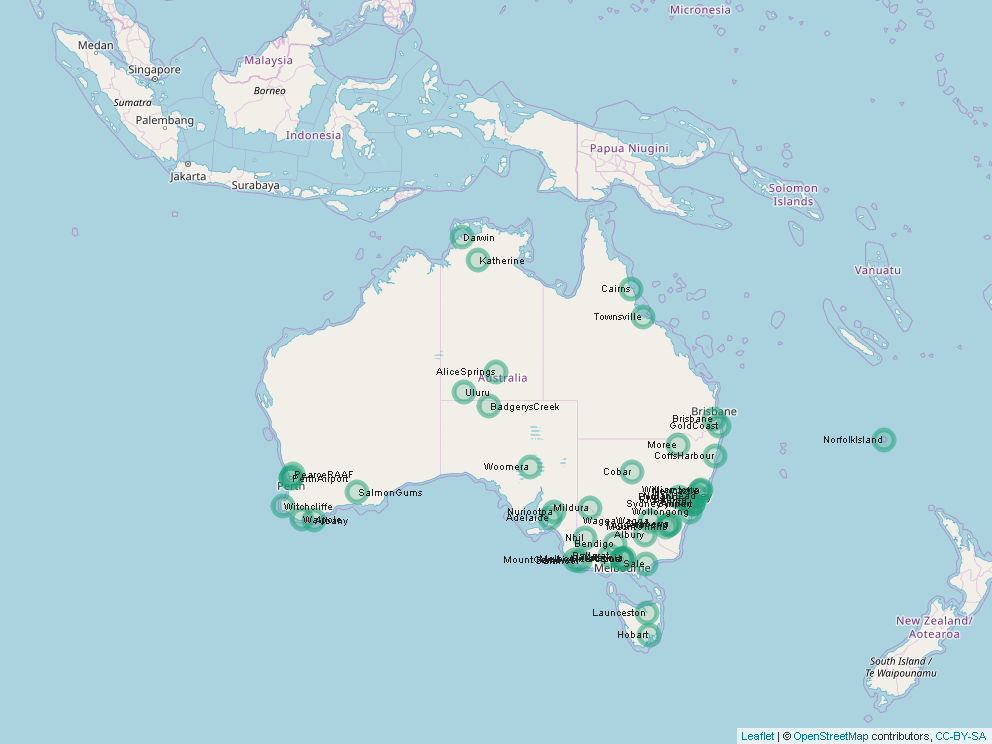
\includegraphics[width=1.1\linewidth]{images/weatherStations} 

}

\caption[Australian Weather Stations]{Australian Weather Stations}\label{fig:map}
\end{figure}
\end{Schunk}

Let's review data summary

\begin{Schunk}
\begin{Sinput}
summary(weatherData)
\end{Sinput}
\begin{Soutput}
#>       Date                Location         MinTemp         MaxTemp     
#>  Min.   :2007-11-01   Canberra:  3418   Min.   :-8.50   Min.   :-4.80  
#>  1st Qu.:2011-01-06   Sydney  :  3337   1st Qu.: 7.60   1st Qu.:17.90  
#>  Median :2013-05-27   Perth   :  3193   Median :12.00   Median :22.60  
#>  Mean   :2013-04-01   Darwin  :  3192   Mean   :12.19   Mean   :23.23  
#>  3rd Qu.:2015-06-12   Hobart  :  3188   3rd Qu.:16.80   3rd Qu.:28.20  
#>  Max.   :2017-06-25   Brisbane:  3161   Max.   :33.90   Max.   :48.10  
#>                       (Other) :122704   NA's   :637     NA's   :322    
#>     Rainfall       Evaporation        Sunshine      WindGustDir   
#>  Min.   :  0.00   Min.   :  0.00   Min.   : 0.00   W      : 9780  
#>  1st Qu.:  0.00   1st Qu.:  2.60   1st Qu.: 4.90   SE     : 9309  
#>  Median :  0.00   Median :  4.80   Median : 8.50   E      : 9071  
#>  Mean   :  2.35   Mean   :  5.47   Mean   : 7.62   N      : 9033  
#>  3rd Qu.:  0.80   3rd Qu.:  7.40   3rd Qu.:10.60   SSE    : 8993  
#>  Max.   :371.00   Max.   :145.00   Max.   :14.50   (Other):86677  
#>  NA's   :1406     NA's   :60843    NA's   :67816   NA's   : 9330  
#>  WindGustSpeed      WindDir9am      WindDir3pm     WindSpeed9am 
#>  Min.   :  6.00   N      :11393   SE     :10663   Min.   :  0   
#>  1st Qu.: 31.00   SE     : 9162   W      : 9911   1st Qu.:  7   
#>  Median : 39.00   E      : 9024   S      : 9598   Median : 13   
#>  Mean   : 39.98   SSE    : 8966   WSW    : 9329   Mean   : 14   
#>  3rd Qu.: 48.00   NW     : 8552   SW     : 9182   3rd Qu.: 19   
#>  Max.   :135.00   (Other):85083   (Other):89732   Max.   :130   
#>  NA's   :9270     NA's   :10013   NA's   : 3778   NA's   :1348  
#>   WindSpeed3pm    Humidity9am      Humidity3pm      Pressure9am    
#>  Min.   : 0.00   Min.   :  0.00   Min.   :  0.00   Min.   : 980.5  
#>  1st Qu.:13.00   1st Qu.: 57.00   1st Qu.: 37.00   1st Qu.:1012.9  
#>  Median :19.00   Median : 70.00   Median : 52.00   Median :1017.6  
#>  Mean   :18.64   Mean   : 68.84   Mean   : 51.48   Mean   :1017.7  
#>  3rd Qu.:24.00   3rd Qu.: 83.00   3rd Qu.: 66.00   3rd Qu.:1022.4  
#>  Max.   :87.00   Max.   :100.00   Max.   :100.00   Max.   :1041.0  
#>  NA's   :2630    NA's   :1774     NA's   :3610     NA's   :14014   
#>   Pressure3pm        Cloud9am        Cloud3pm        Temp9am     
#>  Min.   : 977.1   Min.   :0.00    Min.   :0.0     Min.   :-7.20  
#>  1st Qu.:1010.4   1st Qu.:1.00    1st Qu.:2.0     1st Qu.:12.30  
#>  Median :1015.2   Median :5.00    Median :5.0     Median :16.70  
#>  Mean   :1015.3   Mean   :4.44    Mean   :4.5     Mean   :16.99  
#>  3rd Qu.:1020.0   3rd Qu.:7.00    3rd Qu.:7.0     3rd Qu.:21.60  
#>  Max.   :1039.6   Max.   :9.00    Max.   :9.0     Max.   :40.20  
#>  NA's   :13981    NA's   :53657   NA's   :57094   NA's   :904    
#>     Temp3pm      RainToday     RainTomorrow
#>  Min.   :-5.40   No  :109332   No :110316  
#>  1st Qu.:16.60   Yes : 31455   Yes: 31877  
#>  Median :21.10   NA's:  1406               
#>  Mean   :21.69                             
#>  3rd Qu.:26.40                             
#>  Max.   :46.70                             
#>  NA's   :2726
\end{Soutput}
\end{Schunk}

Next set of plots renders distribution of a few selected features.

\begin{Schunk}
\begin{figure}[H]

{\centering \includegraphics{main_files/figure-latex/feature_distribution-1} 

}

\caption[Observations Distribution]{Observations Distribution}\label{fig:feature_distribution}
\end{figure}
\end{Schunk}

\hypertarget{missing-data}{%
\subsubsection{Missing Data}\label{missing-data}}

Further analysis of data shows that many features are missing. Some data
losses are very significant. We are going to identify what data is
missing and if it is feasible to recover the data.

\begin{Schunk}
\begin{Sinput}
print(sort(colSums(is.na(weatherData)), decreasing = T))
\end{Sinput}
\begin{Soutput}
#>      Sunshine   Evaporation      Cloud3pm      Cloud9am   Pressure9am 
#>         67816         60843         57094         53657         14014 
#>   Pressure3pm    WindDir9am   WindGustDir WindGustSpeed    WindDir3pm 
#>         13981         10013          9330          9270          3778 
#>   Humidity3pm       Temp3pm  WindSpeed3pm   Humidity9am      Rainfall 
#>          3610          2726          2630          1774          1406 
#>     RainToday  WindSpeed9am       Temp9am       MinTemp       MaxTemp 
#>          1406          1348           904           637           322 
#>          Date      Location  RainTomorrow 
#>             0             0             0
\end{Soutput}
\end{Schunk}

To speed up data processing and plot rendering we are going to use a
data sample. For population of 142K observations, 20K sample size would
be sufficient for 99\% confidence level with the confidence interval 1.

\begin{Schunk}
\begin{Sinput}
weatherSample = sample_n(weatherData, 20000)
aggr(weatherSample, numbers = F, prop = T, col = mainPalette, sortVars = T, bars = F, varheight = T)
\end{Sinput}
\begin{figure}[H]

{\centering \includegraphics{main_files/figure-latex/plot_aggr_missing-1} 

}

\caption[Missing Data Summary]{Missing Data Summary}\label{fig:plot_aggr_missing}
\end{figure}
\begin{Soutput}
#> 
#>  Variables sorted by number of missings: 
#>       Variable   Count
#>       Sunshine 0.47890
#>    Evaporation 0.42935
#>       Cloud3pm 0.40110
#>       Cloud9am 0.37700
#>    Pressure9am 0.09755
#>    Pressure3pm 0.09725
#>     WindDir9am 0.06600
#>    WindGustDir 0.06515
#>  WindGustSpeed 0.06465
#>     WindDir3pm 0.02715
#>    Humidity3pm 0.02595
#>        Temp3pm 0.01950
#>   WindSpeed3pm 0.01885
#>    Humidity9am 0.01255
#>   WindSpeed9am 0.00865
#>       Rainfall 0.00795
#>      RainToday 0.00795
#>        Temp9am 0.00600
#>        MinTemp 0.00445
#>        MaxTemp 0.00235
#>           Date 0.00000
#>       Location 0.00000
#>   RainTomorrow 0.00000
\end{Soutput}
\end{Schunk}

As demonstrated in Figure \ref{fig:plot_aggr_missing} \emph{Sunshine},
\emph{Evaporation} and \emph{Clouds} columns safer the loss of data
between \textbf{48\%} and \textbf{38\%}. This is significant! Since we
are dealing with the weather patterns we should be observing cyclical
data patterns. Let's review data distribution of features that damaged
the most.

\begin{Schunk}
\begin{figure}[H]

{\centering \includegraphics{main_files/figure-latex/plot_margin1-1} 

}

\caption[Date/Evaporation Margin Plot]{Date/Evaporation Margin Plot}\label{fig:plot_margin1}
\end{figure}
\end{Schunk}

\begin{Schunk}
\begin{figure}[H]

{\centering \includegraphics{main_files/figure-latex/plot_margin2-1} 

}

\caption[Date/ Sunshine Margin Plot]{Date/ Sunshine Margin Plot}\label{fig:plot_margin2}
\end{figure}
\end{Schunk}

\begin{Schunk}
\begin{figure}[H]

{\centering \includegraphics{main_files/figure-latex/plot_margin3-1} 

}

\caption[Date/ Pressure3pm Margin Plot]{Date/ Pressure3pm Margin Plot}\label{fig:plot_margin3}
\end{figure}
\end{Schunk}

So what do the margin plots tell us? First of all let's take a look at
\emph{Date} axis. The \emph{Date} has been converted to number to ensure
continuous flow of the data . All features we picked exhibit cyclical
pattern as expected. Along the vertical axis we observe the box plot of
the respective feature. \emph{Evaporaton} data is quite remarkable
(Figure \ref{fig: plot_margin1}); it has very narrow distribution and a
lot of so-called outliers. Though forces of nature follow seasonal
patters they often exhibit wide range of seasonal anomalies, which the
plots highlight. The distribution of the missing data of a given feature
is depicted along the horizontal axis. In all three cases the missing
data is randomly distributed along observed date range. Along the
horizontal axis we may see box plots of the date and a given feature.
\emph{Presure9am} ((Figure \ref{fig: plot_margin3})) distributed evenly
across the observed date frame. \emph{Evaporation} and \emph{Sunshine}
exhibit more data losses towards the end of the observed period

Let's examine one more dimension of the missing data, namely features vs
feature vs location

\begin{Schunk}
\begin{figure}[H]

{\centering \includegraphics{main_files/figure-latex/plot_missLocation-1} 

}

\caption[Missing Data By Location]{Missing Data By Location}\label{fig:plot_missLocation}
\end{figure}
\end{Schunk}

Remarkably Figure \ref{fig:plot_missLocation} shows that \textbf{6460}
observations are missing on average per location. Though if we take a
second look at the weather station map \ref{fig:map} we would see that
Mount Gini (the station that miss the most data), Bendigo and Ballarat
are close to Melbrun, where the staff has kept observing data on regular
basis. Newcastle to Sydney and so on\ldots{}

\hypertarget{data-correlation-and-other-observations}{%
\subsubsection{Data correlation and other
observations}\label{data-correlation-and-other-observations}}

Let's examine how the features are correlated to each other. Knowing
weather we can make an accurate prediction that the temperature features
should be highly correlated, as well as pressure, wind speed, clouds and
humidity groups

\begin{Schunk}
\begin{figure}[H]

{\centering \includegraphics[width=1.1\linewidth]{main_files/figure-latex/plot_corr-1} 

}

\caption[Data Correlation]{Data Correlation}\label{fig:plot_corr}
\end{figure}
\end{Schunk}

Figure \ref{fig:plot_corr} confirms our initial guess. This observation
will help us to eliminate redundant features later when we get to the
point of selecting useful predictors for our model

\hypertarget{takeaways-from-data-exploration-excersize}
\item
  \emph{Evaporation} \textbf{43\%}
\item
  \emph{Cloud} group (\textbf{40\%} and \textbf{38\%} respectively)
\item
  The rest of the features exhibit medium to minor data losses, where
  \emph{Pressure} group leads the way with 10\%
\item
  The missing data is distributed randomly over the observed time frame
  (Figures \ref{fig:plot_margin1}, \ref{fig:plot_margin2},
  \ref{fig:plot_margin3})
\item
  We also witnessed that some weather stations recorded less data and
  some were almost prefect at record keeping (Figure
  \ref{fig:plot_missLocation}). Luckily many majority weather stations
  situate relatively close to each other (see figure \ref{fig:map}).
  Thus if a station has data gaps the neighboring station data could be
  used to approximate the missing data with plausible accuracy
\item
  We have also noticed that many features are either positively or
  negatively correlated (Figure \ref{fig:plot_corr}), where
\item
  \emph{MaxTemp}, \emph{Temp3pm} and \emph{Temp9am} exhibits correlation
  of \textbf{0.86} to \textbf{0.98}
\item
  \emph{Pressure9am} and \emph{Pressure3pm} have correlation coefficient
  of \textbf{0.96}
\item
  \emph{Sunshine} and \emph{Cloud} group correlated negatively with
  coefficient of \textbf{-0.7}
\item
  \emph{Rainfall} feature is of particular interest since this is what
  we are trying to predict. Unfortunately it does not demonstrate any
  strong correlations with any other feature
\item
  Doing the data analysis we have also seen seasonal patterns and data
  that fall outside of the normal distribution range by far (outliers).
  Those are anomalies of nature.
\item
  The last but not least the target feature (the value we are trying to
  predict) is unbalanced. so we are dealing with unbalanced data set.
  See Figure \ref{fig:feature_distribution} \emph{RainTomorrow} plot
\end{itemize}

\hypertarget{data-preparation}{%
\subsection{Data Preparation}\label{data-preparation}}

Data exploration confirmed that despite of significant data loss we
should be able to impute data with high degree of plausibility

\hypertarget{datas-imputing}{%
\subsubsection{Datas Imputing}\label{datas-imputing}}

Before we start dealing with missing observations let's do some feature
engineering, which will + improve imputation processing speed + improve
model training performance and hopefully accuracy

First of all let's get rid of \emph{Date} column. Outside of the
presentation it does not carry too mach information. What would be
useful indeed is a feature that captures seasonal observation
fluctuations. That would bee \emph{month} and \emph{day} combined,
giving us year-round (365) days of observations

Secondly we convert categorical features to numbers. But before we do so
we would like to ponder about \emph{Location}. We have couple options
here. Either we convert the locations to the numbers or we can replace
them with the real geographical coordinates. After some deliberation we
can conclude that the coordinates will not add too much knowledge in the
context of the model training. But they will certainly break this
categorical feature (coordinates have 4,6 decimal places, which
effectively make them continuous). So we stick with categories.

This is our original set:

\begin{Schunk}
\begin{Sinput}
str(weatherData)
\end{Sinput}
\begin{Soutput}
#> 'data.frame':    142193 obs. of  23 variables:
#>  $ Date         : Date, format: "2008-12-01" "2008-12-02" ...
#>  $ Location     : Factor w/ 49 levels "Adelaide","Albany",..: 3 3 3 3 3 3 3 3 3 3 ...
#>  $ MinTemp      : num  13.4 7.4 12.9 9.2 17.5 14.6 14.3 7.7 9.7 13.1 ...
#>  $ MaxTemp      : num  22.9 25.1 25.7 28 32.3 29.7 25 26.7 31.9 30.1 ...
#>  $ Rainfall     : num  0.6 0 0 0 1 0.2 0 0 0 1.4 ...
#>  $ Evaporation  : num  NA NA NA NA NA NA NA NA NA NA ...
#>  $ Sunshine     : num  NA NA NA NA NA NA NA NA NA NA ...
#>  $ WindGustDir  : Factor w/ 16 levels "E","ENE","ESE",..: 14 15 16 5 14 15 14 14 7 14 ...
#>  $ WindGustSpeed: int  44 44 46 24 41 56 50 35 80 28 ...
#>  $ WindDir9am   : Factor w/ 16 levels "E","ENE","ESE",..: 14 7 14 10 2 14 13 11 10 9 ...
#>  $ WindDir3pm   : Factor w/ 16 levels "E","ENE","ESE",..: 15 16 16 1 8 14 14 14 8 11 ...
#>  $ WindSpeed9am : int  20 4 19 11 7 19 20 6 7 15 ...
#>  $ WindSpeed3pm : int  24 22 26 9 20 24 24 17 28 11 ...
#>  $ Humidity9am  : int  71 44 38 45 82 55 49 48 42 58 ...
#>  $ Humidity3pm  : int  22 25 30 16 33 23 19 19 9 27 ...
#>  $ Pressure9am  : num  1008 1011 1008 1018 1011 ...
#>  $ Pressure3pm  : num  1007 1008 1009 1013 1006 ...
#>  $ Cloud9am     : int  8 NA NA NA 7 NA 1 NA NA NA ...
#>  $ Cloud3pm     : int  NA NA 2 NA 8 NA NA NA NA NA ...
#>  $ Temp9am      : num  16.9 17.2 21 18.1 17.8 20.6 18.1 16.3 18.3 20.1 ...
#>  $ Temp3pm      : num  21.8 24.3 23.2 26.5 29.7 28.9 24.6 25.5 30.2 28.2 ...
#>  $ RainToday    : Factor w/ 2 levels "No","Yes": 1 1 1 1 1 1 1 1 1 2 ...
#>  $ RainTomorrow : Factor w/ 2 levels "No","Yes": 1 1 1 1 1 1 1 1 2 1 ...
\end{Soutput}
\end{Schunk}

Transformation

\begin{Schunk}
\begin{Sinput}
data = mutate(weatherData,MMDD = as.numeric( format(Date, "%m%d")),Location = unclass(Location), 
              WindGustDir = unclass(WindGustDir),
              WindDir9am = unclass(WindDir9am), WindDir3pm = unclass(WindDir3pm),
              RainToday = unclass(RainToday)-1, RainTomorrow = unclass(RainTomorrow)-1)
data =  subset(data, select = -Date)
\end{Sinput}
\end{Schunk}

Resulting data frame structure:

\begin{Schunk}
\begin{Sinput}
str(data)
\end{Sinput}
\begin{Soutput}
#> 'data.frame':    142193 obs. of  23 variables:
#>  $ Location     : int  3 3 3 3 3 3 3 3 3 3 ...
#>  $ MinTemp      : num  13.4 7.4 12.9 9.2 17.5 14.6 14.3 7.7 9.7 13.1 ...
#>  $ MaxTemp      : num  22.9 25.1 25.7 28 32.3 29.7 25 26.7 31.9 30.1 ...
#>  $ Rainfall     : num  0.6 0 0 0 1 0.2 0 0 0 1.4 ...
#>  $ Evaporation  : num  NA NA NA NA NA NA NA NA NA NA ...
#>  $ Sunshine     : num  NA NA NA NA NA NA NA NA NA NA ...
#>  $ WindGustDir  : int  14 15 16 5 14 15 14 14 7 14 ...
#>  $ WindGustSpeed: int  44 44 46 24 41 56 50 35 80 28 ...
#>  $ WindDir9am   : int  14 7 14 10 2 14 13 11 10 9 ...
#>  $ WindDir3pm   : int  15 16 16 1 8 14 14 14 8 11 ...
#>  $ WindSpeed9am : int  20 4 19 11 7 19 20 6 7 15 ...
#>  $ WindSpeed3pm : int  24 22 26 9 20 24 24 17 28 11 ...
#>  $ Humidity9am  : int  71 44 38 45 82 55 49 48 42 58 ...
#>  $ Humidity3pm  : int  22 25 30 16 33 23 19 19 9 27 ...
#>  $ Pressure9am  : num  1008 1011 1008 1018 1011 ...
#>  $ Pressure3pm  : num  1007 1008 1009 1013 1006 ...
#>  $ Cloud9am     : int  8 NA NA NA 7 NA 1 NA NA NA ...
#>  $ Cloud3pm     : int  NA NA 2 NA 8 NA NA NA NA NA ...
#>  $ Temp9am      : num  16.9 17.2 21 18.1 17.8 20.6 18.1 16.3 18.3 20.1 ...
#>  $ Temp3pm      : num  21.8 24.3 23.2 26.5 29.7 28.9 24.6 25.5 30.2 28.2 ...
#>  $ RainToday    : num  0 0 0 0 0 0 0 0 0 1 ...
#>  $ RainTomorrow : num  0 0 0 0 0 0 0 0 1 0 ...
#>  $ MMDD         : num  1201 1202 1203 1204 1205 ...
\end{Soutput}
\end{Schunk}

To impute the missing data we employ \textbf{MICE} package. Our
imputation strategy is to employ \textbf{Predictive mean matching} model
which is a robust, fast imputation algorithm that works with numeric
values ( this is why we have converted all data to the numeric values)
Lets do a dry run first to see what predictors and methods for each
feature to cure \emph{MICE} software chooses. As before we will be
working with a 20K data sample. Imputation process on the whole set take
about 3 hours and 20 minutes to complete! In addition we let \emph{MICE}
to choose predictors for us running \textbf{quickpred()} method

\begin{Schunk}
\begin{Sinput}
meta = mice(data, maxit = 0, print = FALSE)
weatherSample = sample_n(data, 20000)
methods = meta$method
predictors = quickpred(data) 
\end{Sinput}
\end{Schunk}

Let's review the methods chosen by the software making sure that they
meet our requirements highlighted prior in the imputation strategy
paragraph

\begin{Schunk}
\begin{Sinput}
print(methods)
\end{Sinput}
\begin{Soutput}
#>      Location       MinTemp       MaxTemp      Rainfall   Evaporation 
#>            ""         "pmm"         "pmm"         "pmm"         "pmm" 
#>      Sunshine   WindGustDir WindGustSpeed    WindDir9am    WindDir3pm 
#>         "pmm"         "pmm"         "pmm"         "pmm"         "pmm" 
#>  WindSpeed9am  WindSpeed3pm   Humidity9am   Humidity3pm   Pressure9am 
#>         "pmm"         "pmm"         "pmm"         "pmm"         "pmm" 
#>   Pressure3pm      Cloud9am      Cloud3pm       Temp9am       Temp3pm 
#>         "pmm"         "pmm"         "pmm"         "pmm"         "pmm" 
#>     RainToday  RainTomorrow          MMDD 
#>         "pmm"            ""            ""
\end{Soutput}
\end{Schunk}

The code output above shows that 1 the features without missing data
will not be imputed 2 The imputation targets will all be treated with
\emph{Predictive mean matching} algorithm (``pmm'')

This is exactly what we need. Now let's review the predictors (\emph{The
command output is not included into report to save space })

The matrix of predictors has the predictors in the columns and the
features to be imputed in the rows. If the cell value equals has
\textbf{1} the predictor will be employed in calculations for the
respective imputation target. Surprisingly \textbf{MMDD} is not used
widely to predict the missing data, nether do the \textbf{Location}.

Now we are going to start the imputation process. \textbf{Note: it might
take about 4 - 5 minutes even for a smaple}. We have disabled the output
of the function as we do not want to pollute the report with irrelevant
messages

\begin{Schunk}
\begin{Sinput}
imputed = mice(weatherSample, pred = predictors, meth = methods, seed = 38019,
               nnet.MaxNWts = 2000, printFlag = F)
\end{Sinput}
\end{Schunk}

Now it is time to analyze the imputed values. In general, a good imputed
value is a value that could have been observed had it not been missing.
The MAR assumption can never be tested from the observed data. To check
whether the imputations created by \textbf{MICE} algorithm are plausible
we employ density charts and compare the distribution of the imputed
values vs real observations. Let's do this (\emph{again the plots take
time, patience\ldots{}}).

\begin{Schunk}
\begin{figure}[H]

{\centering \includegraphics[width=1.1\linewidth]{main_files/figure-latex/imputed_density-1} 

}

\caption[Imputed Values Distribution vs Real Observations]{Imputed Values Distribution vs Real Observations}\label{fig:imputed_density}
\end{figure}
\end{Schunk}

Figure \ref{fig:imputed_density} illustrates imputed value distribution
for each imputed feature vs observed data. The fat green line renders
the real data distribution and the thin lines of the other colors the
distribution of imputed values after each imputation cycle (\emph{there
are five of them by default}). Where the last one is yellow. The yellow
line should be shadowing the contour of the green one as close as
possible, which give us an indication that the result of the imputation
is plausible. Looking at the charts we can conclude that the imputation
has been successful! Let's apply imputed values to our sample set and
verify if there are any \emph{NAs} left

\begin{Schunk}
\begin{Sinput}
weatherSample = complete(imputed)
print(colSums(is.na(weatherSample)))
\end{Sinput}
\begin{Soutput}
#>      Location       MinTemp       MaxTemp      Rainfall   Evaporation 
#>             0             0             0             0             0 
#>      Sunshine   WindGustDir WindGustSpeed    WindDir9am    WindDir3pm 
#>             0             0             0             0             0 
#>  WindSpeed9am  WindSpeed3pm   Humidity9am   Humidity3pm   Pressure9am 
#>             0             0             0             0             0 
#>   Pressure3pm      Cloud9am      Cloud3pm       Temp9am       Temp3pm 
#>             0             0             0             0             0 
#>     RainToday  RainTomorrow          MMDD 
#>             0             0             0
\end{Soutput}
\end{Schunk}

Outstanding! There are no missing values. Now we move on to the next
part - model training

\hypertarget{modeling-and-evalutation}{%
\section{Modeling and Evalutation}\label{modeling-and-evalutation}}

Finally we have reached the stage where we can start training and
evaluating classification models. At this point we have clear
understanding of our data. We have gotten rid of the features that did
not present much value. We have filled the gaps in our data set
employing sophisticated imputation technique.

\hypertarget{feature-selection}{%
\subsection{Feature Selection}\label{feature-selection}}

The weather observation data set originally had 24 features. We have
removed \emph{RISK\_MM} and \emph{Date} as explained earlier and added
\emph{MMDD}. Now the data set has 22 features and one label. Let's see
if we can reduce the number of predictors without significant
information loss. This would make our models faster and more
interpretable for users. We shall keep in mind that at the data
exploration phase we have discovered that many features are correlated
(Figure \ref{fig:plot_corr}). hopefully this knowledge will help us
identify and remove redundant features.

Generally speaking feature evaluation methods can be separated into two
groups: those that use the model information and those that do not.
Clearly at this stage the models are not ready. Thus we will be
exploring the methods that do not require model.

This group of the method could be spit further as follows:

\begin{itemize}
\item
  wrapper methods that evaluate multiple models adding and/or removing
  predictors. These are some examples:
\item
  recursive feature elimination
\item
  genetic algorithms
\item
  simulated annealing
\item
  filter methods which evaluate the relevance of the predictors outside
  of the predictive models.
\end{itemize}

The evaluation of various feature selection methods is not in the scope
of this paper. Thus we opt for a recursive feature elimination method
using accuracy as a target metric.

Before we precede any further let's ensure that all categorical values
get converted to factors. This is useful for dimentiality reduction
algorithms and model training.

\begin{Schunk}
\begin{Sinput}
weatherSample = mutate(weatherSample, Location = as.factor(unclass(Location)), WindGustDir = as.factor(unclass(WindGustDir)),
              WindDir9am = as.factor(unclass(WindDir9am)), WindDir3pm = as.factor(unclass(WindDir3pm)),
              RainToday = as.factor(unclass(RainToday)), RainTomorrow = as.factor(unclass(RainTomorrow)))
\end{Sinput}
\end{Schunk}

Let's run feature selection algorithm

\begin{Schunk}
\begin{Sinput}
predictors = subset(weatherSample,select = -RainTomorrow)
label = weatherSample[,22]

# run the RFE algorithm
rfePrediction = rfe(predictors, label, sizes=c(1:22), 
                    rfeControl = rfeControl(functions=rfFuncs, method="cv", number=3))
print(rfePrediction)
\end{Sinput}
\begin{Soutput}
#> 
#> Recursive feature selection
#> 
#> Outer resampling method: Cross-Validated (3 fold) 
#> 
#> Resampling performance over subset size:
#> 
#>  Variables Accuracy  Kappa AccuracySD KappaSD Selected
#>          1   0.8246 0.3697   0.006184 0.02093         
#>          2   0.8238 0.4029   0.005341 0.01846         
#>          3   0.8363 0.4626   0.005281 0.01611         
#>          4   0.8407 0.5123   0.005726 0.01779         
#>          5   0.8477 0.5344   0.005467 0.01799         
#>          6   0.8499 0.5430   0.004719 0.01427         
#>          7   0.8506 0.5448   0.005481 0.01816         
#>          8   0.8513 0.5433   0.004741 0.01548         
#>          9   0.8525 0.5489   0.005507 0.01359         
#>         10   0.8505 0.5447   0.006654 0.02123         
#>         11   0.8501 0.5476   0.003881 0.01026         
#>         12   0.8518 0.5502   0.005392 0.01569         
#>         13   0.8533 0.5542   0.005360 0.01558         
#>         14   0.8543 0.5569   0.004677 0.01544         
#>         15   0.8529 0.5518   0.003675 0.01413         
#>         16   0.8528 0.5532   0.003679 0.01562         
#>         17   0.8534 0.5547   0.002974 0.01497         
#>         18   0.8542 0.5585   0.003763 0.01142         
#>         19   0.8534 0.5542   0.003598 0.01229         
#>         20   0.8546 0.5554   0.004635 0.01411         
#>         21   0.8545 0.5549   0.004744 0.01550         
#>         22   0.8555 0.5571   0.005470 0.01664        *
#> 
#> The top 5 variables (out of 22):
#>    Humidity3pm, Sunshine, WindGustSpeed, Location, Pressure3pm
\end{Soutput}
\end{Schunk}

\begin{Schunk}
\begin{figure}[H]

{\centering \includegraphics[width=1.1\linewidth]{main_files/figure-latex/plot_feature_selection-1} 

}

\caption[Number of Predictors vs Accuracy]{Number of Predictors vs Accuracy}\label{fig:plot_feature_selection}
\end{figure}
\end{Schunk}

Figure \ref{fig:plot_feature_selection} shows that accuracy peaks at
around 7 predictors and then around 12. It reaches maximum when all
features are used, but the accuracy increases negligibly. Thus we can
stick to the first 7. Here is the list of features ordered by
importance:

\begin{Schunk}
\begin{Sinput}
print(predictors(rfePrediction))
\end{Sinput}
\begin{Soutput}
#>  [1] "Humidity3pm"   "Sunshine"      "WindGustSpeed" "Location"     
#>  [5] "Pressure3pm"   "Cloud3pm"      "Rainfall"      "Pressure9am"  
#>  [9] "WindDir3pm"    "WindGustDir"   "Humidity9am"   "MinTemp"      
#> [13] "Cloud9am"      "WindSpeed3pm"  "WindDir9am"    "RainToday"    
#> [17] "Temp9am"       "Temp3pm"       "Evaporation"   "WindSpeed9am" 
#> [21] "MaxTemp"       "MMDD"
\end{Soutput}
\end{Schunk}

\hypertarget{data-upsampling}{%
\subsubsection{Data Upsampling}\label{data-upsampling}}

There is one more step before we get to the model training. As shown in
Figure \ref{fig:feature_distribution} our data set is unbalanced. This
could cause model overfiting. So let's split the data into the training
and testing sets and up-sample the training set

\begin{Schunk}
\begin{Sinput}
set.seed(1608)
splitIdx = createDataPartition(weatherSample$RainTomorrow, p=0.7, list = F)  # 70% training data
trainData = weatherSample[splitIdx, ]
testData = weatherSample[-splitIdx, ]

set.seed(590045)
columns = colnames(trainData)
trainData = upSample(x = trainData[, columns[columns != "RainTomorrow"] ], y = trainData$RainTomorrow, list = F, yname = "RainTomorrow")
# verify data balance in training balanced set
print(table(trainData$RainTomorrow))
\end{Sinput}
\begin{Soutput}
#> 
#>     0     1 
#> 10891 10891
\end{Soutput}
\end{Schunk}

As we can see the training set is balanced.

Thus we have prepared our training and test data sets. We have
identified the most important features. We are ready to work on the
prediction models

\hypertarget{decision-tree-model}{%
\subsection{Decision Tree Model}\label{decision-tree-model}}

\hypertarget{naive-bayes-model}{%
\subsection{Naive Bayes Model}\label{naive-bayes-model}}

\hypertarget{random-forest-model}{%
\subsection{Random Forest Model}\label{random-forest-model}}

\hypertarget{logistic-regression-model}{%
\subsection{Logistic Regression Model}\label{logistic-regression-model}}

\hypertarget{model-comparison}{%
\subsection{Model Comparison}\label{model-comparison}}

\hypertarget{model-deployment}{%
\section{Model Deployment}\label{model-deployment}}

\hypertarget{conclusion}{%
\section{Conclusion}\label{conclusion}}

\hypertarget{bibliography}{%
\section{Bibliography}\label{bibliography}}


\address{%
Sumaira Afzal\\
York University School of Continuing Studies\\
\\
}


\address{%
Viraja Ketkar\\
York University School of Continuing Studies\\
\\
}


\address{%
Murlidhar Loka\\
York University School of Continuing Studies\\
\\
}


\address{%
Vadim Spirkov\\
York University School of Continuing Studies\\
\\
}


